%%
% This is an Overleaf template for presentations
% using the TUM Corporate Desing https://www.tum.de/cd
%
% For further details on how to use the template, take a look at our
% GitLab repository and browse through our test documents
% https://gitlab.lrz.de/latex4ei/tum-templates.
%
% The tumbeamer class is based on the beamer class.
% If you need further customization please consult the beamer class guide
% https://ctan.org/pkg/beamer.
% Additional class options are passed down to the base class.
%
% If you encounter any bugs or undesired behaviour, please raise an issue
% in our GitLab repository
% https://gitlab.lrz.de/latex4ei/tum-templates/issues
% and provide a description and minimal working example of your problem.
%%

%\makeatletter
%\def\input@path{{../beamer/}}
%\makeatother

\documentclass[
  german,            % define the document language (english, german)
  aspectratio=169,    % define the aspect ratio (169, 43)
  % handout=2on1,       % create handout with multiple slides (2on1, 4on1)
  % partpage=false,     % insert page at beginning of parts (true, false)
  % sectionpage=true,   % insert page at beginning of sections (true, false)
]{tumbeamer}


% load additional packages
\usepackage{booktabs}
\usepackage{graphicx}
\usepackage{tikz}
\usepackage{url}
\usepackage{pgfplots}
\usepackage{hyperref}
\usepackage{pmboxdraw}
\usepackage{float}
\usepackage{listings}
\usepackage{circuitikz}
%\usepackage[european]{circuitikz}
\usepackage{babel}[ngerman]
\usepackage{csquotes}[autostyle]
\usepackage[useregional]{datetime2}

% image path
\graphicspath{ {./resources/} }

% presentation metadata
\title{Übung 10: Caches}
\subtitle{Einführung in die Rechnerarchitektur}
\author{Niklas Ladurner}

\institute{\theChairName\\\theDepartmentName\\\theUniversityName}
\date{\DTMdisplaydate{2024}{1}{5}{-1}}

\footline{\insertauthor~|~\insertshorttitle~|~\insertshortdate}


% macro to configure the style of the presentation
\TUMbeamersetup{
  title page = TUM tower,         % style of the title page
  part page = TUM toc,            % style of part pages
  section page = TUM toc,         % style of section pages
  content page = TUM more space,  % style of normal content pages
  tower scale = 1.0,              % scaling factor of TUM tower (if used)
  headline = TUM threeliner,      % which variation of headline to use
  footline = TUM default,         % which variation of footline to use
  % configure on which pages headlines and footlines should be printed
  headline on = {title page},
  footline on = {every page, title page=false},
}

% available frame styles for title page, part page, and section page:
% TUM default, TUM tower, TUM centered,
% TUM blue default, TUM blue tower, TUM blue centered,
% TUM shaded default, TUM shaded tower, TUM shaded centered,
% TUM flags
%
% additional frame styles for part page and section page:
% TUM toc
%
% available frame styles for content pages:
% TUM default, TUM more space
%
% available headline options:
% TUM empty, TUM oneliner, TUM twoliner, TUM threeliner, TUM logothreeliner
%
% available footline options:
% TUM empty, TUM default, TUM infoline


\begin{document}

\maketitle

\begin{frame}[c]{}{}
  \begin{center}
    \LARGE  Durchzählen!
  \end{center}
\end{frame}

\begin{frame}[c]{}{}
  \begin{center}
    \LARGE  Keine Garantie für die Richtigkeit der Tutorfolien: Bei Unklarheiten/Unstimmigkeiten
    haben VL/ZÜ-Folien Recht!
  \end{center}
\end{frame}

\begin{frame}[fragile, c]{Speicherarten}{}
  \begin{itemize}
    \item Static RAM (SRAM): schnell, aber geringe Kapazität (Flipflops)
    \item Dynamic RAM (DRAM): langsam, dafür aber günstig in großer Kapazität herstellbar (Kondensatoren)
    \item Vorteile/Nachteile der beiden Arten sind einfache Klausuraufgabe!
  \end{itemize}

\end{frame}

\begin{frame}[fragile, c]{Caches}{}
  \begin{itemize}
    \item \enquote{Zwischenstation} $\;$zwischen Registern (sehr schnell, sehr klein) und Hauptspeicher (sehr langsam, sehr groß)
    \item Idee: Häufig genutzte Daten im Cache zwischenspeichern
    \item heutzutage meist L1/L2/L3-Caches: Caches aufsteigender Größe, aber absteigender Zugriffszeit 
  \end{itemize}
\end{frame}


\begin{frame}[c, fragile]{Caches}{}
  \begin{itemize}
    \item Hit: Datum liegt im Cache, Miss: Datum nicht im Cache, muss erst aus Hauptspeicher geholt werden
    \item Ziel: möglichst hohe Hitrate (Hits/Anfragen), d.h. häufig genutzte Daten liegen im Cache
    \item zeitliche Lokalität: Zugriff auf x $\rightarrow$ wschl. Zugriff auf x in Zukunft
    \item räumliche Lokalität: Zugriff auf x $\rightarrow$ Zugriff auf Daten in der Nähe (oft durch Cacheline abgedeckt)
    \item Formeln für CPU-Time und Memory Access Rate kennen $\rightarrow$ war letztes Jahr Klausuraufgabe
    \item Ersetzungsstrategien auch wichtig (FIFO, LRU, LFU)
  \end{itemize}
\end{frame}

\begin{frame}[c, fragile]{Cachestrukturen}
  \begin{itemize}
    \item Direct Mapped Cache: direkte Abbildung Hauptspeicheradresse $\rightarrow$ Cache-Adresse (jede Cachezeile kann nur an einer bestimmten Stelle im Cache stehen)
    \item Fully Associative Cache: eine Cacheline kann an einer beliebigen Stelle im Cache stehen
    \item Set Associative Cache (Mengenassoziativer Cache): Aufteilung in sog. Sets, Set wird durch Adresse bestimmt, aber innerhalb des Sets kann die Cacheline an einer bel. Stelle stehen
    \item Tag: Identifikation der Cacheline im Set, Index: bestimmt Set im Cache, Offset: bestimmt Datum innerhalb einer Cacheline
    \item Adresse eines Datums wird aufgeteilt!
  \end{itemize}
\end{frame}


\begin{frame}[c, fragile]{Cachestrukturen}
  \begin{center}
    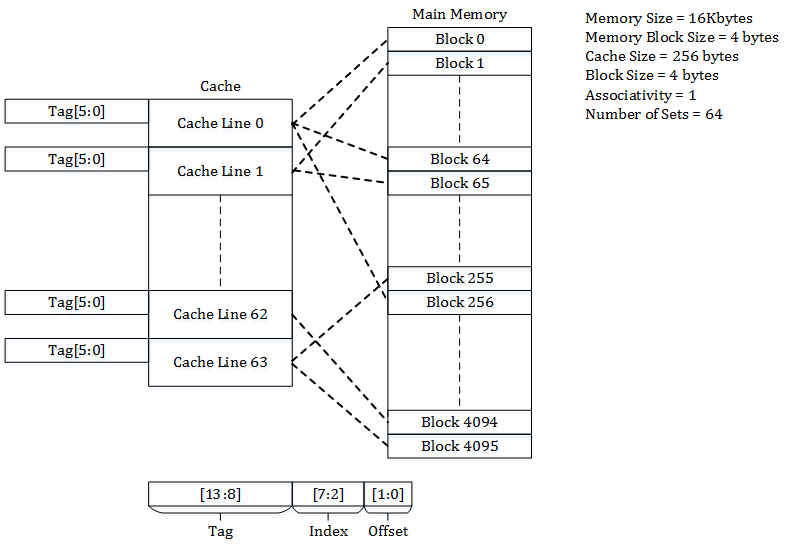
\includegraphics[width=0.65\textwidth]{w10_cache.png}
  \end{center}
  \begin{center}
    \tiny Quelle: \href{https://en.wikipedia.org/wiki/Cache_placement_policies}{Wikipedia}
  \end{center}
\end{frame}

\begin{frame}[c, fragile]{Ein paar Formeln$\ldots$}
  Für einen n-assoziativen Cache (jeweils n Cachezeilen in seinem Set):
  \vspace{0.25cm}
  \begin{itemize}
    \item $\textrm{Anzahl Cache-Lines}=\frac{\textrm{Cachegröße}}{\textrm{Cachezeilengröße}}$
    \item $\textrm{Anzahl Cache-Sets}=\frac{\textrm{Anzahl Cache-Lines}}{\textrm{n}}$
    \item $\textrm{Anzahl Index-Bits}=\lceil\log_2(\textrm{Anzahl Cache-Sets})\rceil$
    \item $\textrm{Anzahl Offset-Bits}=\lceil\log_2(\textrm{Cachezeilengröße})\rceil$
    \item $\textrm{Anzahl Tag-Bits}= \textrm{Anzahl Adressbits} - \textrm{Anzahl Index-Bits} - \textrm{Anzahl Offset-Bits}$
  \end{itemize}
\end{frame}


\begin{frame}[c]{}{}
  \begin{center}
    \LARGE Fragen?
  \end{center}
\end{frame}

\begin{frame}[c, fragile]{Artemis-Hausaufgaben}{}
  \begin{itemize}
    \item H10 - 4-Fach-Assoziativ bis 14.01.2024 23:59 Uhr
    \item Werte in einem Cache einfügen (+ Ersetzungen), Abgabe im Textformat
    \item gut machbar, Tests geben wieder vor der Deadline volles Feedback
  \end{itemize}
\end{frame}

\begin{frame}[fragile, c]{Links}{}
  \begin{itemize}
    \item Zulip: \href{https://zulip.in.tum.de/#narrow/stream/1917-ERA-Tutorium---Mi-1600-MI4}{\enquote{ERA Tutorium - Mi-1600-MI4}}
    bzw. \href{https://zulip.in.tum.de/#narrow/stream/1940-ERA-Tutorium---Fr-1100-MW2}{\enquote{ERA Tutorium - Fr-1100-MW2}}
    \item \href{https://en.wikipedia.org/wiki/Cache_placement_policies}{Wikipedia zu Caches}
    \item \href{https://www.elektronik-kompendium.de/sites/com/0309291.htm}{Elektronik-Kompendium zu Caches}
    \item \href{https://www.elektronik-kompendium.de/sites/com/0309191.htm}{Elektronik-Kompendium zu SRAM/DRAM}
  \end{itemize}
\end{frame}

\maketitle

\end{document}
